\documentclass[11pt]{article}
\usepackage{algorithm}
\usepackage[noend]{algpseudocode}
% Shared preamble for the qurl-theory reports.
% Build either report from this folder with:  latexmk -pdf <file>.tex
% (or: pdflatex <file>; bibtex <file>; pdflatex <file>; pdflatex <file>)

\usepackage[T1]{fontenc}
\usepackage{lmodern}
\usepackage[margin=1in]{geometry}
\usepackage{microtype}
\usepackage{amsmath,amssymb,amsthm,mathtools}
\usepackage{booktabs,tabularx,array}
\usepackage{enumitem}
\usepackage[dvipsnames]{xcolor}
\usepackage[authoryear,round]{natbib}
\usepackage{xurl}  % lets long URLs break anywhere (loads url)

% Allow a line break (without an inserted hyphen) after each \_ in text, so long file names can wrap.
\makeatletter
\DeclareRobustCommand{\_}{\ifmmode\nfss@text{\textunderscore}\else\textunderscore\allowbreak\fi}
\makeatother
\usepackage[colorlinks=true,linkcolor=NavyBlue,citecolor=ForestGreen,urlcolor=RoyalBlue]{hyperref}
\usepackage[capitalise,noabbrev]{cleveref}

% ---- theorem-like environments (defined after cleveref so shared counters get the right names)
\theoremstyle{plain}
\newtheorem{theorem}{Theorem}
\newtheorem{proposition}[theorem]{Proposition}
\newtheorem{lemma}{Lemma}
\newtheorem{corollary}{Corollary}
\theoremstyle{definition}
\newtheorem{definition}{Definition}
\newtheorem*{assumptionU}{Assumption U}
\theoremstyle{remark}
\newtheorem{remark}{Remark}

% ---- status tags (robust, so they can appear in section titles and the table of contents)
\DeclareRobustCommand{\statustag}[2]{\textsf{\footnotesize\textcolor{#1}{[#2]}}}
\DeclareRobustCommand{\tagchecked}{\statustag{ForestGreen}{checked}}
\DeclareRobustCommand{\tagproved}{\statustag{RoyalBlue}{proved}}
\DeclareRobustCommand{\tagderived}{\statustag{RoyalBlue}{derived}}
\DeclareRobustCommand{\tagconj}{\statustag{BurntOrange}{conjecture}}
\DeclareRobustCommand{\tagopen}{\statustag{BrickRed}{open}}

% ---- research-problem headings (numbered P1, P2, ... by hand, listed in the table of contents)
\newcommand{\researchproblem}[2]{%
  \subsubsection*{#1.\ #2}\addcontentsline{toc}{subsubsection}{#1.\ #2}}

% ---- math and text macros
\newcommand{\E}{\mathbb{E}}
\newcommand{\R}{\mathbb{R}}
\newcommand{\N}{\mathbb{N}}
\newcommand{\Z}{\mathbb{Z}}
\newcommand{\Unif}{\mathcal{U}}
\DeclareMathOperator{\Var}{Var}
\DeclareMathOperator{\Corr}{Corr}
\DeclareMathOperator{\clip}{clip}
\DeclareMathOperator{\diag}{diag}
\DeclareMathOperator{\sgn}{sign}
\DeclareMathOperator{\fracpart}{frac}
\DeclareMathOperator{\rms}{rms}
\newcommand{\KL}{\mathrm{KL}}
\newcommand{\TV}{\mathrm{TV}}
\newcommand{\script}[1]{\texttt{sanity\_checks/\allowbreak#1}}
\newcolumntype{L}{>{\raggedright\arraybackslash}X}
\setlist{itemsep=2pt,topsep=4pt}

% ---- layout: avoid overfull lines from unbreakable math/citations; ragged-right bibliography
\setlength{\emergencystretch}{1.5em}
\renewcommand{\bibfont}{\raggedright}

\usepackage{graphicx}  % figures: standalone TikZ files in figures/, built with tectonic
\usepackage{flafter}   % a float never appears before the point where it is defined

\newcommand{\pold}{\pi_{\mathrm{old}}}
\newcommand{\thold}{\theta_{\mathrm{old}}}
\newcommand{\qthold}{\hat\theta_{\mathrm{old}}}
\newcommand{\Ehat}{\widehat{\mathbb E}}
\algrenewcommand\algorithmiccomment[1]{\hfill{\footnotesize$\triangleright$~#1}}

\title{QuRL, Explained:\\Reinforcement Learning with Quantized Rollouts}
\author{Explainer for the QuRL research notes (draft)}
\date{12 November 2026}

\begin{document}
\maketitle

\paragraph{Scope.} A short explanation of QuRL \citep{li2026qurl}, from version~1 of arXiv:2602.13953 (February 2026, the only version), whose LaTeX source was downloaded fresh from arXiv on 12 November 2026. \Cref{sec:problem} states the problem, \cref{sec:background} explains PPO, GRPO and where the time goes, and \cref{sec:algorithm} gives the algorithm. The research notes (\texttt{research\_problems.tex} and the P1 notes) point to the line of \cref{alg:qurl} where each of their problems arises.

% =====================================================================================
\section{The problem QuRL addresses}\label{sec:problem}
Reinforcement learning with verifiable rewards (RLVR) trains a reasoning LLM by letting it answer questions, checking the answers automatically and reinforcing the good ones. Every training step generates responses (the \emph{rollout}), scores them and updates the model.
\begin{itemize}
\item \textbf{The bottleneck is generation.} Responses are decoded one token at a time, so the rollout takes up to about 70\% of training time, and more with long chains of thought (\cref{sec:bottleneck}).
\item \textbf{QuRL's idea.} Generate the rollouts with an 8-bit copy of the model (weights and activations in INT8 or FP8) and train the full-precision (FP) model as usual. The paper reports 20--80\% faster rollout.
\item \textbf{The catch.} The responses now come from a slightly different model than the one being trained.
  \begin{enumerate}
  \item \emph{Off-policy data.} The 8-bit policy $\mu$ samples; the FP policy is trained. PPO and GRPO assume the two are the same, and used naively they collapse or lose accuracy (\cref{sec:decoupled}).
  \item \emph{The ``weight update problem'' (the paper's claim).} An RL step moves each weight by about $10^{-7}$--$10^{-6}$, much less than the 8-bit rounding error, so, the paper argues, the 8-bit copy barely changes from step to step (\cref{sec:uaq}).
  \end{enumerate}
\item \textbf{QuRL's answer.} For the first problem, decoupled PPO with truncated importance sampling (TIS, as in FlashRL, \citealp{yao2025flashrl}) and a new \emph{Adaptive Clipping Range} (ACR); for the second, \emph{Update-Aware Quantization} (UAQ). \Cref{fig:loop} shows one step.
\end{itemize}

\begin{figure}[t]
\centering
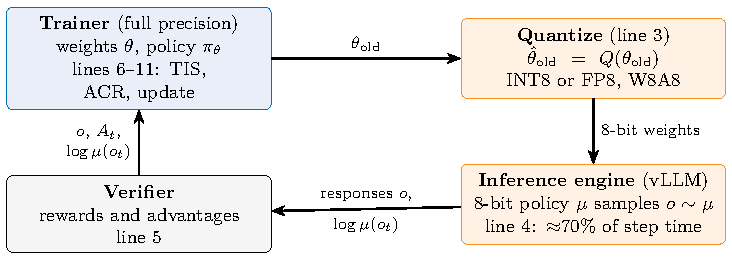
\includegraphics{figures/fig_loop.pdf}
\caption{One QuRL step. The trainer keeps full-precision weights; each step it sends an 8-bit copy to the inference engine, which generates the responses. Line numbers refer to \cref{alg:qurl}. In all figures, blue marks full precision and orange 8-bit.}
\label{fig:loop}
\end{figure}

% =====================================================================================
\section{Background: PPO, GRPO and the rollout bottleneck}\label{sec:background}

\subsection{RL for LLMs}\label{sec:rl}
For a prompt $q$, the policy $\pi_\theta$ (the LLM) samples a response $o=(o_1,\dots,o_T)$ one token at a time, $o_t\sim\pi_\theta(\cdot\mid q,o_{<t})$. A verifier returns a reward $v(q,o)\in\{0,1\}$, for example whether the final answer is correct. Training raises the expected reward with policy-gradient steps,
\[
\nabla_\theta J(\theta)=\E\Bigl[\textstyle\sum_t A_t\,\nabla_\theta\log\pi_\theta(o_t\mid q,o_{<t})\Bigr],
\]
where the \emph{advantage} $A_t$ says how much better than expected the response turned out. A KL penalty keeps $\pi_\theta$ close to a reference model $\pi_{\mathrm{ref}}$, usually the starting model.

\subsection{PPO}\label{sec:ppo}
PPO \citep{schulman2017ppo} reuses one batch of rollouts for several minibatch updates. Since $\pi_\theta$ drifts away from the policy $\pold$ that generated the batch, each token is weighted by the ratio $R_t=\pi_\theta(o_t)/\pold(o_t)$ (contexts omitted from here on), and the ratio is clipped:
\begin{equation}\label{eq:ppo}
J_{\mathrm{PPO}}(\theta)=\Ehat_t\Bigl[\min\bigl(R_tA_t,\ \clip(R_t,1-\epsilon,1+\epsilon)\,A_t\bigr)\Bigr],
\end{equation}
where $\Ehat_t$ averages over the tokens of the batch. The clip is a \emph{trust region}: a token with $A_t>0$ stops contributing gradient once it has become $1+\epsilon$ times more likely, and one with $A_t<0$ once its probability has fallen to $1-\epsilon$ times its old value (typically $\epsilon=0.2$); \cref{fig:clip}(a,~b) plots both cases. PPO estimates $A_t$ with a learned critic (a value model) and generalized advantage estimation \citep{schulman2016gae}.

\subsection{GRPO}\label{sec:grpo}
GRPO \citep{shao2024deepseekmath} drops the critic. For each prompt it samples a \emph{group} of $G$ responses and gives every token of response $i$ the same advantage,
\begin{equation}\label{eq:grpo}
A_{i,t}=\frac{v_i-\mathrm{mean}(v_1,\dots,v_G)}{\mathrm{std}(v_1,\dots,v_G)},
\end{equation}
where $v_i$ is the reward of response $i$ (\cref{fig:clip}(c) gives an example). The objective is \eqref{eq:ppo}, averaged over each response's tokens and then over the group, minus $\beta\,\KL(\pi_\theta\|\pi_{\mathrm{ref}})$. DAPO \citep{yu2025dapo}, one of QuRL's test settings, is a GRPO variant with an asymmetric clip ($\epsilon_{\mathrm{low}}=0.2$, $\epsilon_{\mathrm{high}}=0.28$) and no KL term.

\begin{figure}[htbp]
\centering
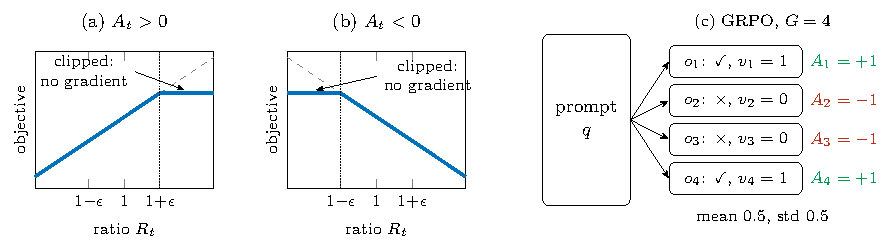
\includegraphics{figures/fig_clip.pdf}
\caption{(a,~b) PPO's per-token objective as a function of the ratio $R_t$; the dashed line is where the unclipped $R_tA_t$ would continue. Once a token's probability has moved by more than $\epsilon$ in the direction its advantage favours, the objective is flat and the token gives no gradient. (c) GRPO's advantages for a group of four responses to one prompt: correct answers get $A>0$ and are made more likely, wrong ones get $A<0$.}
\label{fig:clip}
\end{figure}

\subsection{Where the bottleneck arises}\label{sec:bottleneck}
A PPO or GRPO step has three phases (\cref{fig:time}): (1) the \emph{rollout} generates the responses, $G$ per prompt, in an inference engine such as vLLM \citep{kwon2023vllm}; (2) \emph{scoring} computes the log-probabilities of all sampled tokens under $\pold$ (and $\pi_{\mathrm{ref}}$, and the critic's values); (3) the \emph{update} runs forward and backward passes over minibatches.

\begin{figure}[htbp]
\centering
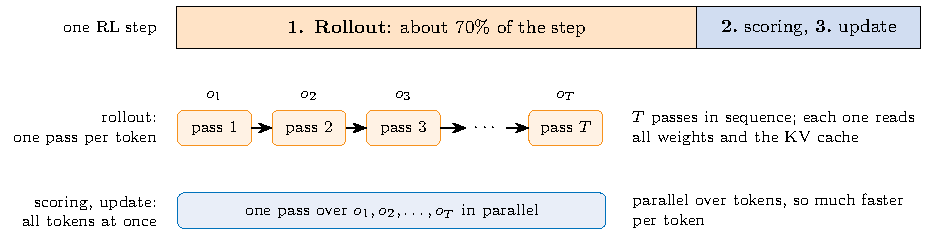
\includegraphics{figures/fig_time.pdf}
\caption{Where the time of one RL step goes. The rollout produces one token per forward pass; scoring and the update process all tokens of a response in one pass. QuRL speeds up the rollout by running it in 8 bits.}
\label{fig:time}
\end{figure}

Phases 2 and 3 process all tokens of a response at once. The rollout needs one forward pass per generated token, each reading all weights and the KV cache, and reasoning responses run to thousands of tokens, so it dominates: about 70\% of the step in QuRL's measurements. Quantizing the weights and activations to 8 bits lets the engine use INT8 or FP8 matrix multiplications, which is where QuRL's speedup comes from. The paper finds that larger models gain more (+20--30\% throughput at 7B, +70--90\% at 32B with INT8) and attributes this to large models being limited by matrix multiplications and small ones by memory I/O.

One more fact matters below. The inference engine and the training framework compute probabilities with different kernels, so even in BF16 the sampling policy differs slightly from the trained one. FlashRL \citep{yao2025flashrl} corrects for this with TIS (\cref{sec:tis}); quantization makes the gap much larger.

% =====================================================================================
\section{The QuRL algorithm}\label{sec:algorithm}

\subsection{Notation}\label{sec:notation}
\begin{center}\small
\begin{tabularx}{\linewidth}{@{}l L@{}}
\toprule
Symbol & Meaning\\
\midrule
$\theta$, $\pi_\theta$ & FP weights being trained, and their policy\\
$\thold$, $\pold$ & FP weights and policy when the batch was generated (the \emph{proximal} policy)\\
$\qthold=Q(\thold)$, $\mu$ & 8-bit copy of $\thold$, and its policy, which generates the batch (the \emph{behavior} policy)\\
$R_t=\pi_\theta(o_t)/\pold(o_t)$ & PPO ratio: how far training has moved from $\pold$\\
$\rho_t=\pold(o_t)/\mu(o_t)$ & proximal-to-behavior ratio: the quantization mismatch on token $o_t$\\
$w_t=\min(\rho_t,C)$ & TIS weight, capped at $C$\\
$r_t=\min(1,C/\rho_t)$ & truncation factor, so that $w_t=r_t\rho_t$; $r_t<1$ only where $\rho_t>C$\\
$A_t$, $\epsilon$, $s$ & advantage, clip parameter, UAQ scale ($s=1.5$)\\
\bottomrule
\end{tabularx}
\end{center}
The paper writes $\pi_{\qthold}$ for $\mu$ and $\pi_{\thold}$ for $\pold$; the research notes write $\mu_k$ and $\pi_k$ for the two at step $k$.

\subsection{Pseudocode}\label{sec:pseudocode}
\Cref{alg:qurl} shows QuRL with GRPO, the paper's main presentation. With PPO, line~\ref{line:adv} uses a critic and line~\ref{line:update} also updates it. All quantities with subscript $t$ are per token of every response.

\begin{algorithm}[tb]
\caption{QuRL (one training run)}\label{alg:qurl}
\begin{algorithmic}[1]
\Require FP weights $\theta$, reference $\pi_{\mathrm{ref}}$, 8-bit quantizer $Q$ (INT8 or FP8, W8A8), UAQ scale $s$, TIS cap $C$, clip $\epsilon$
\State UAQ, once: $W_{Q,K,V}\gets W_{Q,K,V}/s$; RMSNorm gain before them $\gamma\gets s\gamma$ \Comment{same FP model}\label{line:uaq}
\For{each RL step}
  \State $\thold\gets\theta$;\quad $\qthold\gets Q(\thold)$, loaded into the inference engine \Comment{re-quantize}\label{line:quant}
  \State For each prompt: sample $G$ responses $o\sim\mu=\pi_{\qthold}$; keep $\log\mu(o_t)$ \Comment{8-bit rollout}\label{line:rollout}
  \State Rewards $v_i$ from the verifier; advantages $A_t$ by \eqref{eq:grpo}\label{line:adv}
  \State $\log\pold(o_t)$ from the FP trainer \Comment{one forward pass}\label{line:prox}
  \State $\rho_t\gets\pold(o_t)/\mu(o_t)$;\quad $w_t\gets\min(\rho_t,C)$;\quad $r_t\gets\min(1,C/\rho_t)$ \Comment{TIS}\label{line:tis}
  \For{each epoch and minibatch}
    \State $R_t\gets\pi_\theta(o_t)/\pold(o_t)$\label{line:ratio}
    \State $J(\theta)\gets\Ehat_t\bigl[w_t\min\bigl(R_tA_t,\ \clip\bigl(R_t,1-\epsilon,\tfrac{1+\epsilon}{r_t}\bigr)A_t\bigr)\bigr]-\beta\,\KL(\pi_\theta\|\pi_{\mathrm{ref}})$ \Comment{ACR}\label{line:acr}
    \State $\theta\gets$ one optimizer step that increases $J(\theta)$\label{line:update}
  \EndFor
\EndFor
\end{algorithmic}
\end{algorithm}

\subsection{Quantized rollout (lines~\ref{line:quant}--\ref{line:rollout})}\label{sec:rollout}
\begin{itemize}
\item \textbf{What is quantized.} The weights of every linear layer (one absmax scale per output channel) and their input activations (one scale per token), to INT8 or FP8 with round-to-nearest. The matrix multiplications run on vLLM's 8-bit kernels. The KV cache stays in BF16, because FP8 KV caching gave no speedup in the vLLM version used.
\item \textbf{When.} Every step, the freshly updated FP weights are quantized again from scratch and loaded into the engine (line~\ref{line:quant}). There is no calibration: GPTQ-style methods would be too slow to run every step, and quantization-aware training would add a mismatch between the engines.
\item \textbf{What the trainer sees.} The trainer keeps and updates the FP weights and never trains the 8-bit copy. The engine returns each sampled token's log-probability under $\mu$ (line~\ref{line:rollout}), which TIS and ACR use later.
\end{itemize}

\subsection{Off-policy data and decoupled PPO (lines~\ref{line:prox}, \ref{line:ratio} and~\ref{line:acr})}\label{sec:decoupled}
The batch was sampled by $\mu$, while PPO's ratio assumes it was sampled by $\pold$. The paper first tries two naive objectives:
\begin{itemize}
\item \textbf{Anchor on $\mu$:} use $\pi_\theta/\mu$ as the PPO ratio. Training collapses within a few steps; the share of clipped tokens jumps to 1.5\%, then drops to zero.
\item \textbf{Ignore $\mu$:} use $\pi_\theta/\pold$ as if $\pold$ had sampled the batch. Training is stable but ends below BF16, because the gradient is biased.
\end{itemize}
QuRL adopts \emph{decoupled PPO} \citep{hilton2022batch,fu2025areal}, which separates the policy that sampled the data (the behavior policy $\mu$) from the policy that anchors the trust region (the proximal policy $\pold$):
\begin{equation}\label{eq:decoupled}
J_{\mathrm{dec}}(\theta)=\Ehat_{o\sim\mu}\Bigl[\rho_t\,\min\bigl(R_tA_t,\ \clip(R_t,1-\epsilon,1+\epsilon)\,A_t\bigr)\Bigr].
\end{equation}
The weight $\rho_t$ corrects for sampling from $\mu$ instead of $\pold$ (importance sampling), and the clip keeps $\pi_\theta$ close to the FP policy $\pold$ rather than to the noisy $\mu$ (\cref{fig:policies}). Computing $\log\pold$ (line~\ref{line:prox}) is one FP forward pass over the batch, the same pass that standard PPO implementations use for their old log-probabilities.

\begin{figure}[htbp]
\centering
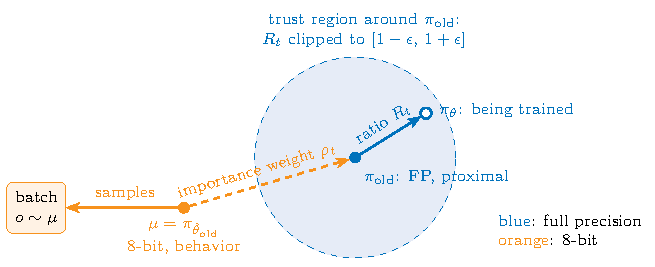
\includegraphics{figures/fig_policies.pdf}
\caption{The three policies of decoupled PPO (schematic). The batch comes from the 8-bit policy $\mu$. The importance weight $\rho_t=\pold/\mu$ reweights it to the FP policy $\pold$, and the trust region for the ratio $R_t=\pi_\theta/\pold$ is centred on $\pold$, not on $\mu$.}
\label{fig:policies}
\end{figure}

\subsection{Truncated importance sampling (line~\ref{line:tis})}\label{sec:tis}
Where $\mu$ gives a token a much lower probability than $\pold$, $\rho_t$ is huge (the paper sees values up to $10^5$), and so is the gradient. TIS, as used in FlashRL \citep{yao2025flashrl}, caps the weight at $C$:
\begin{equation}\label{eq:tis}
J_{\mathrm{TIS}}(\theta)=\Ehat_{o\sim\mu}\Bigl[\min(\rho_t,C)\,\min\bigl(R_tA_t,\ \clip(R_t,1-\epsilon,1+\epsilon)\,A_t\bigr)\Bigr].
\end{equation}
Capping is the same as replacing $\mu$ by the truncated behavior policy $\max(\mu,\pold/C)$: much lower variance, at the price of some bias (\cref{fig:tisacr}(a)). The behavior log-probabilities come straight from the engine, so TIS adds no computation.

\subsection{Adaptive clipping range (lines~\ref{line:tis} and~\ref{line:acr})}\label{sec:acr}
\begin{itemize}
\item \textbf{The failure.} TIS trains well for about 500 steps. In longer runs the gap between the behavior and proximal policies, $\KL(\mu\|\pold)$, keeps growing (from 0.002 to 0.025 after about 1{,}000 steps in the paper), and training collapses.
\item \textbf{The diagnosis.} Write the TIS weight as $w_t=r_t\rho_t$ and move the factor $r_t\le1$ inside the clip:
\[
r_t\,\clip(R_t,1-\epsilon,1+\epsilon)=\clip\bigl(r_tR_t,\ r_t(1-\epsilon),\ r_t(1+\epsilon)\bigr).
\]
On truncated tokens, TIS therefore clips the scaled ratio $r_tR_t$ to a range shrunk by $r_t$. For $A_t>0$ the upper bound falls below $1+\epsilon$, and the paper argues that this clips positive-advantage tokens too early.
\item \textbf{The fix.} ACR keeps the upper bound of the scaled ratio at $1+\epsilon$; that is, it clips $R_t$ at $(1+\epsilon)/r_t$:
\begin{equation}\label{eq:acr}
J_{\mathrm{ACR}}(\theta)=\Ehat_{o\sim\mu}\Bigl[w_t\min\Bigl(R_tA_t,\ \clip\Bigl(R_t,\,1-\epsilon,\,\frac{1+\epsilon}{r_t}\Bigr)A_t\Bigr)\Bigr].
\end{equation}
Since $(1+\epsilon)/r_t=(1+\epsilon)\max(1,\rho_t/C)$, tokens with $\rho_t\le C$ are treated exactly as in TIS. Tokens with $\rho_t>C$, which the 8-bit model under-samples, get a wider upper bound, so those with positive advantage keep being pushed up (\cref{fig:tisacr}(b)). The weights $w_t$ and the lower bound are unchanged.
\end{itemize}

\begin{figure}[htbp]
\centering
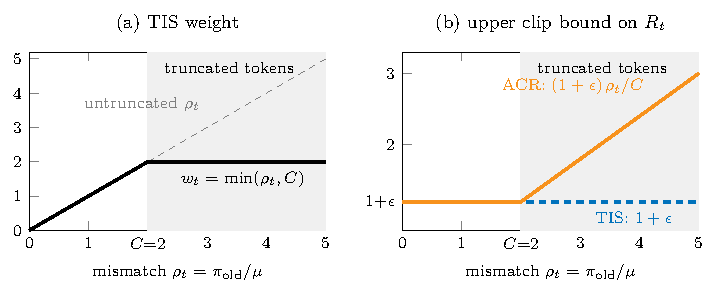
\includegraphics{figures/fig_tis_acr.pdf}
\caption{TIS and ACR as functions of the mismatch $\rho_t$, drawn for $C=2$ and $\epsilon=0.2$. (a)~TIS caps the importance weight at $C$. (b)~ACR raises the upper clip bound on the truncated tokens (shaded) and equals TIS elsewhere.}
\label{fig:tisacr}
\end{figure}

\subsection{Update-aware quantization (line~\ref{line:uaq})}\label{sec:uaq}
\begin{itemize}
\item \textbf{The paper's argument.} One step changes a weight by about $\eta g\approx10^{-7}$--$10^{-6}$ (learning rate $\eta=10^{-6}$, gradient entries 0.1--1), while 8-bit rounding moves it by about $|\theta|/2^b$, with weights of size 0.001--0.1. Re-quantization should then hide almost every update; in the paper's words, it ``masks nearly all weight updates, effectively freezing the quantized model'' (\cref{fig:uaq}(a)).
\item \textbf{The method.} Before RL, rescale the query, key and value projections and the RMSNorm gain that feeds them:
\begin{equation}\label{eq:uaq}
W_{Q,K,V}\to W_{Q,K,V}/s,\qquad \gamma\to s\gamma,\qquad\text{so that}\quad (W/s)(sX)=WX.
\end{equation}
The FP model computes the same function (\cref{fig:uaq}(b)), and nothing changes at run time. The paper argues that the rounding error of $W/s$ is $s$ times smaller while the gradient with respect to $W/s$ is $s$ times larger (it is computed with the $s$-times larger activations), an $s^2$ gain in the ratio of update to error. It uses $s=1.5$; in its ablation, $s=2$ or a 1.5--2$\times$ larger global learning rate did worse.
\item \textbf{Caveat (our analysis).} QuRL's quantizers scale per output channel and per token, so the scales move with the tensors. The rescaling therefore cancels exactly in the 8-bit product, and training the rescaled weights equals training the original ones with per-layer learning rates ($\times s$ on Q/K/V and $\div s$ on the norm gain under Adam). This is research problem P1 (P1 theory note, Theorems~1 and~2).
\end{itemize}

\begin{figure}[htbp]
\centering
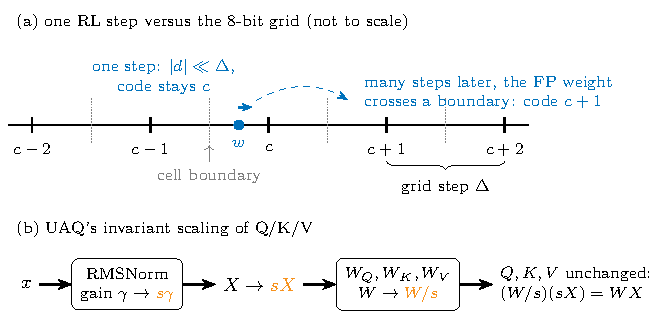
\includegraphics{figures/fig_uaq.pdf}
\caption{(a) The weight update problem, not to scale: one step moves an FP weight by far less than the grid step $\Delta$, so its 8-bit code usually stays the same. The FP weight keeps the change, and the code flips once the accumulated change crosses a cell boundary. (b) UAQ's invariant scaling: the RMSNorm gain is multiplied by $s$ and the Q/K/V weights are divided by $s$, so the FP layer computes the same output.}
\label{fig:uaq}
\end{figure}

\subsection{What the paper reports}\label{sec:reports}
\begin{center}\small
\begin{tabularx}{\linewidth}{@{}L c c c c@{}}
\toprule
Setting (model; metric) & BF16 & 8-bit, uncorrected & FlashRL & QuRL\\
\midrule
PPO on GSM8K (Qwen2.5-0.5B-Instruct; accuracy), INT8 & 55.35 & 48.78 & 51.40 & 53.55\\
\quad same, FP8 & 55.35 & 0.0 & 53.60 & 54.28\\
DAPO (Qwen2.5-Math-7B; AIME24 Avg@32), INT8 & 31.67 & ${\approx}0$ & 30.29 & 30.63 / 31.25\\
\quad same, FP8 & 31.67 & ${\approx}0$ & 32.60 & 33.12 / 33.27\\
GRPO on DeepScaleR (R1-Distill-Qwen-1.5B; mean Avg@32 over 5 benchmarks), INT8 & 56.40 & 52.31 & 53.80 & 54.79 / 55.48\\
\bottomrule
\end{tabularx}
\end{center}
QuRL entries are without / with UAQ; the GSM8K runs use learning rate $10^{-5}$ and no UAQ. FlashRL is decoupled PPO with TIS. No error bars are reported. With INT8, rollout throughput rises by 20--30\% at 7B and by 70\% (A100) to 90\% (H100) at 32B.

\bibliographystyle{plainnat}
\bibliography{refs}

\end{document}
